\chapter{Missing Values}
\label{missing_values}
\thispagestyle{empty}

A ciascun utente sono associati due tipi di proprietà: il profilo e i like. I like sono ovviamente variabili da un individuo all'altro, né a senso trattare l'assenza di un \textit{mi piace} su un certo contenuto come valore mancante. In generale, parliamo quindi di valori mancanti solo per i dati di profilo, dove sono raccolte le informazioni biografiche dell'utente. Una ulteriore ragione per dare maggior peso all'assenza di informazione di profilo rispetto ai like è il ruolo che questi dati rivestiranno nell'analisi. Mentre i like sono fondamentali per produrre il clustering, gli attributi di profilo sono essenziali per interpretare i cluster. Una volta tracciati i cluster siamo in grado di capire quali interessi accomunano le persone; ma, assumendo di non avere altre fonti di informazione, senza i dati del profilo non è possibile caratterizzare questi gruppi, descrivere con le variabili della segmentazione tradizionale le persone che ne fanno parte, ed il risultato perde significativamente valore.\\
Tra gli algoritmi che abbiamo selezionato, solo Cesna \cite{cesna} è insensibile ai valori mancanti; per tutti gli altri è stato necessario produrre una versione completa dei dati. \`E tuttavia necessario provare a intuire la causa dell'assenza dei dati per stabilire quale meccanismo di completamento dell'informazione ne accresca, e non riduca, la qualità. In questa fase, abbiamo fatto ricorso a tre soluzioni: rimuovere l'individuo con missing values (la riga del dataset), rimuovere integralmente l'attributo (la colonna del dataset) o inferire il valore laddove assente. La prima soluzione è consigliabile quando l'individuo è così povero di informazione da non produrre alcun beneficio all'analisi. Le cause di tale penuria sono disparate: un profilo sostanzialmente inattivo, non aggiornato né mantenuto dal momento della creazione; l'irrilevanza dell'informazione nell'ottica del proprietario del profilo; la riservatezza, tale che o l'utente non ha appositamente inserito l'informazione nel profilo o i permessi in nostro possesso non sono sufficienti per accedere ai dati esistenti. Richiamando la terminologia introdotta in \autoref{subsec:missing_value}, inattività e irrilevanza ricadono nella tipologia MCAR, in quanto non vi è alcuna connessione tra il valore dell'attributo mancante e il fatto che non sia stato inserito. La riservatezza invece è generalmente MNAR; sebbene un individuo preoccupato per la propria privacy possa essere portato a occultare indiscriminatamente i propri dati (MCAR), è ragionevole e conservativo assumere che il non pubblicare una informazione possa dipendere dal valore dell'attributo per l'utente considerato. Per meglio comprendere i dati che avevamo raccolto e discriminare tra questi due casi, abbiamo studiato la relazione nel dataset tra la completezza dei dati biografici e il numero di like, assumendo quest'ultimo come una misura della partecipazione dell'utente al social network e dell'attività del profilo; i risultati sono mostrati in \autoref{fig:profile_vs_likes}. L'ipotesi alla base di questo studio, da confermare o smentire, è che un profilo povero di informazione sia anche poco attivo, quindi povero di like.
\begin{figure}[h]
    \centering
    \begin{subfigure}[b]{0.47\textwidth}
		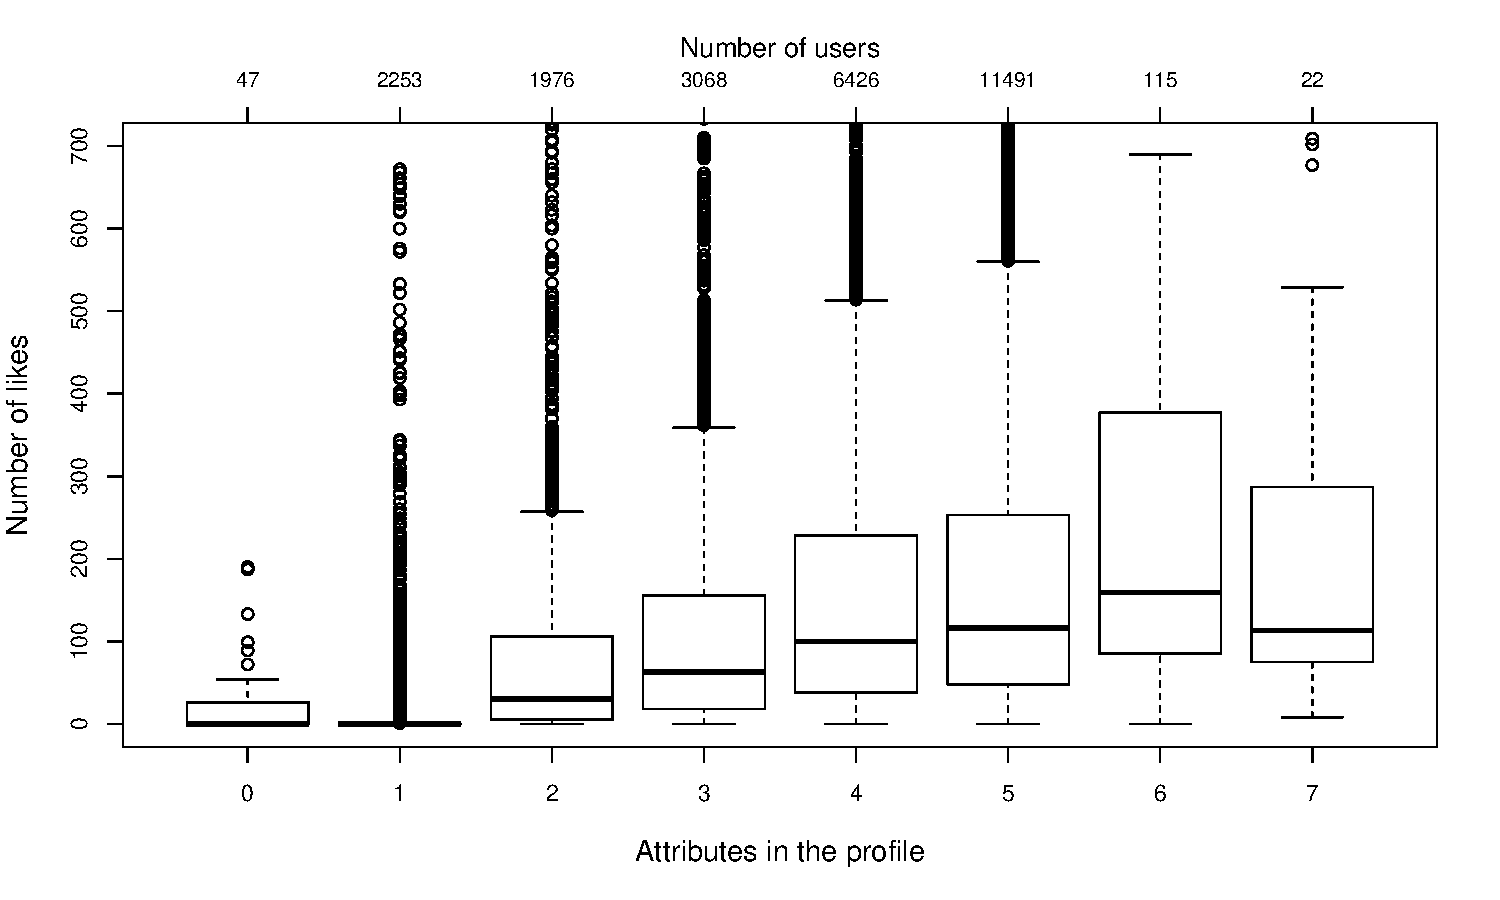
\includegraphics[width=\textwidth]{pictures/profile_vs_likes.pdf}
		\caption{dataset completo}
		\label{fig:profile_vs_likes_users}
	\end{subfigure}
	\hfill
    %add desired spacing between images, e. g. ~, \quad, \qquad, \hfill etc.
    %(or a blank line to force the subfigure onto a new line)
	\begin{subfigure}[b]{0.47\textwidth}
		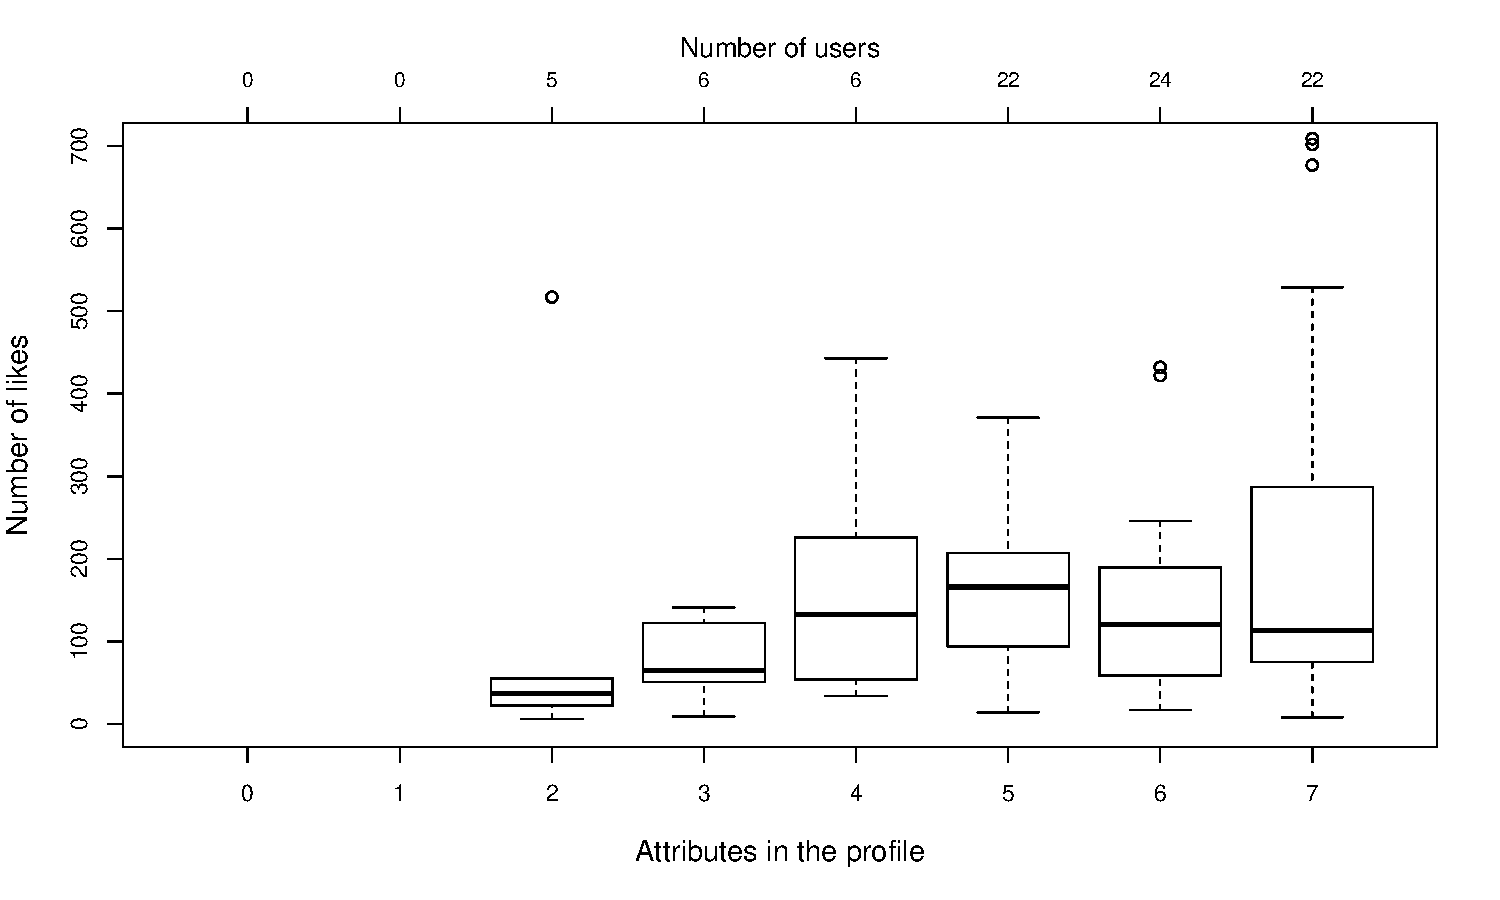
\includegraphics[width=\textwidth]{pictures/profile_vs_likes_dau.pdf}
		\caption{utenti dell'applicazione facebook}
		\label{fig:profile_vs_likes_daus}
	\end{subfigure}
	\caption{Relazione tra il numero di attributi e like nel profilo utente}
	\label{fig:profile_vs_likes}
\end{figure}\\
A sinistra (\autoref{fig:profile_vs_likes_users}), la relazione è valutata sull'intera popolazione; a destra sui soli utenti dell'applicazione. Sulle ascisse riportiamo il numero di attributi specificati dall'utente: da 0, profilo completamente vuoto, a 7\footnote{Sebbene il profilo contenga effettivamente nove attributi, abbiamo accorpato i tre campi (opzionali) relativi all'educazione in un unico attributo, assente se nessuno dei tre gradi di istruzione è specificato}, informazione piena. Si può osservare che esiste una moderata correlazione tra le grandezze sugli assi, la completezza del profilo e il numero di like, che crescono di pari passo. Fa eccezione l'ultima colonna, che tuttavia contiene solo utenti dell'applicazione ed è infatti identica nei due grafici. La differenza è che solo per questi ultimi, gli utenti dell'applicazione, siamo certi di osservare il profilo completo di ogni informazione inserita, a prescindere dalle impostazioni di visibilità. Per tutti gli altri utenti infatti la quantità di informazione che possiamo osservare dipende dai permessi concessi all'utente che li ha aggiungi al grafo (vedi liste di amici).
Data la vastità del dataset, oltre 25000 nodi, è estremamente inverosimile che nessuno tra gli utenti che non hanno partecipato alla raccolta dei dati abbia un profilo completo, e possiamo quindi percepire i limiti dell'informazione indiretta. Si aggiunge pertanto un'altra causa di assenza dei dati, legata stavolta al punto di vista dal quale osserviamo il grafo sociale. Questa connessione tra i due aspetti del profilo ci ha permesso di rimuovere gli utenti sostanzialmente privi di dati biografici senza degradare l'informazione complessiva nel dataset.\\
La seconda soluzione, rimuovere integralmente una dimensione, è necessaria quando l'attributo è mancante per una significativa porzione della popolazione: in questo scenario, rimuovere gli individui privi dell'attributo sarebbe un spreco di informazione e non è nemmeno disponibile sufficiente informazione reale per inferire i valori mancanti. Dai risultati in \autoref{table:missing_values} si evince che gli attributi \textit{orientamento sessuale} e \textit{stato sentimentale} sono specificati da una estrema minoranza di utenti, certamente troppo pochi per applicare una procedura di imputazione; pertanto sono stati rimossi dal dataset.
\begin{table}[h]
\resizebox{0.8\textwidth}{!}{\begin{minipage}{\textwidth}
\begin{tabular}{| c | c | c | c | c | c | c | r}
\multicolumn{1}{c}{genere}
 &  \multicolumn{1}{c}{età}
 & \multicolumn{1}{c}{\specialcell[t]{luogo di\\nascita}}
 & \multicolumn{1}{c}{\specialcell[t]{luogo di\\residenza}}
 & \multicolumn{1}{c}{educazione}
 & \multicolumn{1}{c}{\specialcell[t]{orientamento\\sessuale}}
 & \multicolumn{1}{c}{\specialcell[t]{stato\\sentimentale}}
 & \multicolumn{1}{c}{}
 \tabularnewline
\cline{1-7}
0.0078 & 0.3253 & 0.2802 & 0.2364 & 0.2429 & 0.9913 & 0.9984 & dataset\tabularnewline
\cline{1-7}
0 & 0 & 0.2 & 0.1882 & 0.1412 & 0.5412 & 0.5186 & DAU\tabularnewline
\cline{1-7}
\end{tabular}
\caption{Distribuzione dei valori mancanti per attributo}
\label{table:missing_values}
\end{minipage} }
\end{table}
Una analisi a parte merita l'educazione, che descrive l'aver frequentato la scuola superiore, un corso universitario triennale e magistrale. Nonostante si tratti di campi opzionali---un individuo può certamente non aver frequentato l'università---e il valore si assesti ben al di sotto della media italiana\footnote{Dal Quarto Rapporto sulla coesione sociale in Italia, il 37.8\% dei giovani tra i 18 e 24 anni ha conseguito al massimo la licenza media}, poiché i nostri dati descrivono principalmente studenti universitari e la loro cerchia di  amici, risulta inspiegata una percentuale tanto alta di assenza di qualsivoglia livello di istruzione superiore (\autoref{table:missing_values}). Questo lascia pensare che vi sia un significativa incidenza di missing values anche per questo attributo, ed un stima per difetto si ottiene dall'incidenza dei dati incongruenti: individui che frequentano studi universitari senza aver inserito nel proprio profilo i gradi di istruzione inferiori (\autoref{table:missing_values_education}).
\begin{table}[h]
\resizebox{0.8\textwidth}{!}{\begin{minipage}{\textwidth}
\begin{tabular}{l | c | c | c | r}
 \multicolumn{1}{c}{} 
 & \multicolumn{1}{c}{scuola superiore}
 & \multicolumn{1}{c}{università triennale}
 & \multicolumn{1}{c}{università specialistica}
 & \multicolumn{1}{c}{}
 \tabularnewline
\cline{2-4}
\multirow{2}{*}{\centering dataset} & 0.3232 & 0.4176 & 0.9297 & non specificato \tabularnewline
\cline{2-4}
& 0.0794 & 0.0120 & 0 & incongruente \tabularnewline
\cline{2-4}
\cline{2-4}
\multirow{2}{*}{\centering DAU} & 0.2824 & 0.2 & 0.8353 & non specificato \tabularnewline
\cline{2-4}
& 0.1412 & 0 & 0 & incongruente \tabularnewline
\cline{2-4}
\end{tabular}
\caption{Distribuzione dei valori mancanti per ciascun grado di istruzione}
\label{table:missing_values_education}
\end{minipage} }
\end{table}\\
Ad esempio, l'attributo \textit{scuola superiore} è assente dal 28\% dei profili degli utenti che hanno utilizzato la nostra applicazione, ma ben la metà di questi hanno pubblicato la frequenza di corsi universitari pur senza citare quelli precedenti.\\
In ultimo, i valori possono essere dedotti tramite imputazione. Come discusso precedentemente, i dati mancanti sono anche MNAR e per essi non esiste una procedura univoca di inferenza. Abbiamo deciso pertanto di sviluppare una procedura di imputazione ad hoc, facendo leva sull'omofilia nella rete. Per ciascun individuo con missing value abbiamo considerato gli utenti a cui è connesso nel grafo delle amicizie, e stimato il valore dell'attributo mancante da quello dei suoi vicini. A questo punto, la stima può avvenire con uno dei metodi definiti in letteratura: media, hot-deck, regressione etc. Un problema di questo metodo è che non sfrutta tutta l'informazione nel dataset per completare i valori mancanti ma si avvale soltanto dei vicini. Quando un individuo non ha un vicinato sufficientemente ampio, o i vicini a loro volta non possiedono l'attributo mancante nel soggetto, l'imputazione non ha basi sufficientemente solide per essere affidabile. Per questa ragione abbiamo ulteriormente rimosso dal dataset i nodi poveri di attributi di profilo e debolmente connessi al grafo. Con le due fasi di rimozione dei dati impuri, la dimensione del dataset è drasticamente calata; abbiamo quantificato la perdita di informazione in \autoref{table:cleaned_dataset_statistics}.
\begin{table}[h]
\centering
\begin{tabular}{l | c | c | c |}
 \multicolumn{1}{c}{} 
 & \multicolumn{1}{c}{nodi}
 & \multicolumn{1}{c}{archi \textit{friend}}
 & \multicolumn{1}{c}{archi \textit{like}}
 \tabularnewline
\cline{2-4}
originale (con MV) & 25853 & 975\hspace{2pt}382 & 4\hspace{2pt}391\hspace{2pt}494 \tabularnewline
\cline{2-4}
completo (senza MV) & 16336 & 710\hspace{2pt}711 & 3\hspace{2pt}131\hspace{2pt}019 \tabularnewline
\cline{1-4}
decremento assoluto & 9517 & 264\hspace{2pt}671 & 1\hspace{2pt}260\hspace{2pt}475 \tabularnewline
\cline{2-4}
decremento percentuale & 36.81\% & 27.14\% & 28.7\% \tabularnewline
\cline{2-4}
\end{tabular}
\caption{Perdita di informazione durante l'imputazione dei valori mancanti}
\label{table:cleaned_dataset_statistics}
\end{table}\\
%Missingness by attribute
%interested_in 0.9913379
%gender 0.007874636
%hometown 0.280652
%location 0.2375384
%birthday 0.3262855
%relationship_status 0.9983857
%education 0.2437594
%missingness for education
%HS			College		GR Sc		
%0.3231751 	0.4175526 	0.9296795
%True missing
%HS			College		GR Sc
%0.0794157	0.01204819	0
missing values introduced by transformations (coordinates missing after geocoding)